
The Neural Collaborative Filtering (NCF) approach \cite{he2017neural} is tightly related to the Matrix Factorization (MF) method \cite{koren2009matrix}, and provides a framework that is able to express MF and also generalize it.
Instead of simply ``combining'' the user and item latent vectors using a fixed inner product, NCF utilizes a multi-layer neural network architecture that learns the interaction function from the data, and thus, increases the expressiveness of the MF model.

An instance of the NCF framework takes as input two binary one-hot encoded vectors, one for the user, and one the item, and passes them through an embedding layer, i.e. a fully connected layer that projects the sparse representations onto dense vectors.
The obtained user and item embeddings can be viewed as the user and item latent vectors, respectively.
These vectors are then fed into a multi-layer neural network architecture, the output layer of which computes a predicted score $\hat{y}_{ui}$, for the specific user-item interaction.
This score represents how likely the item i is relevant to the user u.

Considering the one-class nature of implicit feedback, the value of $y_{ui}$ is being viewed as a label, where 1 means item relevant to u, and 0 otherwise.
Therefore, training is performed by minimizing the standard binary cross-entropy loss (a.k.a. negative log loss) between $\hat{y}_{ui}$ and its target value $y_{ui}$.
It should be noted, that in order to treat the problem as a binary classification problem and use the aforementioned loss function, negative instances are also required.
These instances are uniformly sampled from the unobserved interactions in each iteration.

In the paper \cite{he2017neural}, three instantiations of the NCF approach are considered, namely, the Generalized Matrix Factorization (GMF), the Multi-Layer Perceptron (MLP), and the Neural Matrix Factorization (NeuMF).
We briefly discuss them below.

\textbf{GMF:} Considering that the output of the embedding layer is the user and item latent vectors $p_u$ and $q_i$, respectively, we can define the mapping function of the first NCF layer as the element-wise product $p_u \odot q_i$.
We can then choose the output layer to be:
\begin{equation}
    \hat{y}_{ui} = \alpha_{out}(\vec{h}^{\T}(\vec{p}_{\idxu} \odot \vec{q}_{\idxi}))\label{eq:gmf}
\end{equation}
where $a_{out}$ and $h$ denote the activation function and affine transformation weights, respectively.
Setting $a_{out}$ to the identity and enforcing $h$ to be a uniform vector of 1, we can exactly recover the MF model.
In the GMF model, the authors set $a_{out}$ to the sigmoid function and learn the values of $h$ from the data with the log loss, effectively generalizing the MF approach.

\textbf{MLP:}
Instead of computing the element-wise product of the user and item latent vector, in a neural network framework it seems definitely intuitive to concatenate them, and then feed them into a standard MLP to learn the user-item interaction function.
In this way, much more flexibility and nonlinearity can be incorporated to the model, compared to the GMF approach, and increased expressiveness can be achieved. 
In \cite{he2017neural}, the authors utilize a tower pattern for the layers, halving the layer size for each successive layer.
As activation function the use ReLU in the middle layers, and sigmoid in the output layer.

\textbf{NeuMF:}
In the NeuMF model, the authors fuse the GMF and MLP approaches into a single architecture (see Fig. \ref{fig:neumf}) in an attempt to combine the linearity of MF and non-linearity of MLP, and thus to be able to better capture complex user-item interactions.
They even add more flexibility to the fused model by allowing GMF and MLP to learn separate embeddings.
In the last layer, the outputs of GMF and MLP are concatenated and are being fed into a sigle neuron with a sigmoid activation function.

\begin{figure}[t]
    \centering
    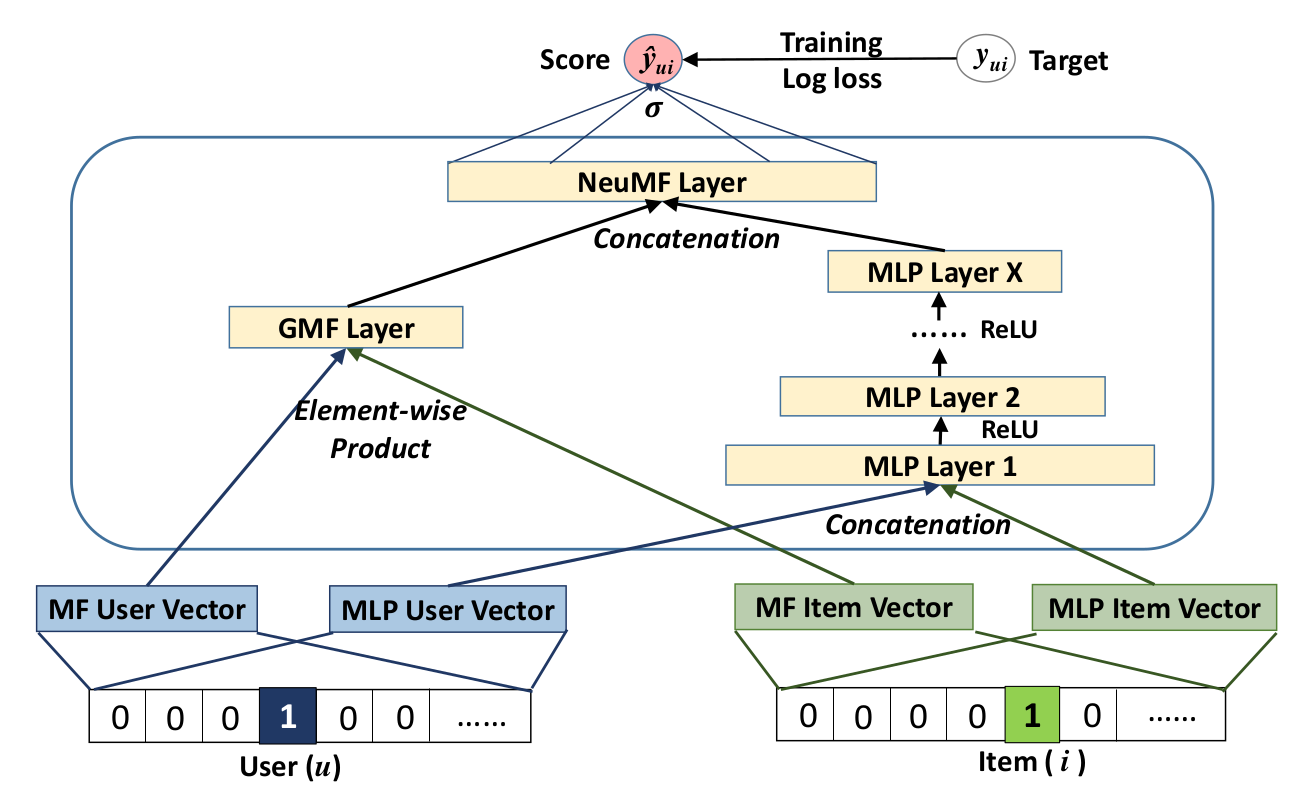
\includegraphics[width=0.8\linewidth]{images/neumf.png}
    \caption{Neural matrix factorization model taken from \cite{he2017neural}}
    \label{fig:neumf}
\end{figure}

%%% Local Variables:
%%% mode: latex
%%% TeX-master: "../../report"
%%% End:
